%
% teil2.tex -- Beispiel-File für teil2 
%
% (c) 2020 Prof Dr Andreas Müller, Hochschule Rapperswil
%
% !TEX root = ../../buch.tex
% !TEX encoding = UTF-8
%
\section{Bildliche Darstellung der Flussüberquerung
\label{schwimmen:section:bildliche_darstellung}}
\rhead{Teil 2}



Die Gleichung \ref{eq:angle} beschreibt das Verhältnis \(\frac{dy}{dx}\) für die Schwimmrichtung der schwimmenden Person, um die optimale Flussüberquerung zu erreichen. 

In \ref{fig:river_pfrofiles} ist eine Visuelle-Darstellung für die Flussüberquerung. Es ist zu sehen das die Person am Uferrand viel nach oben schwimmt und dan, in der mitte des Flusses fast keine Änderung in \(y\)-Richtung macht sondern nur in \(x\)-Richtung.




%papers/schwimmen/
\begin{figure}
    \centering
    \begin{subfigure}{0.48\textwidth}
        \centering
        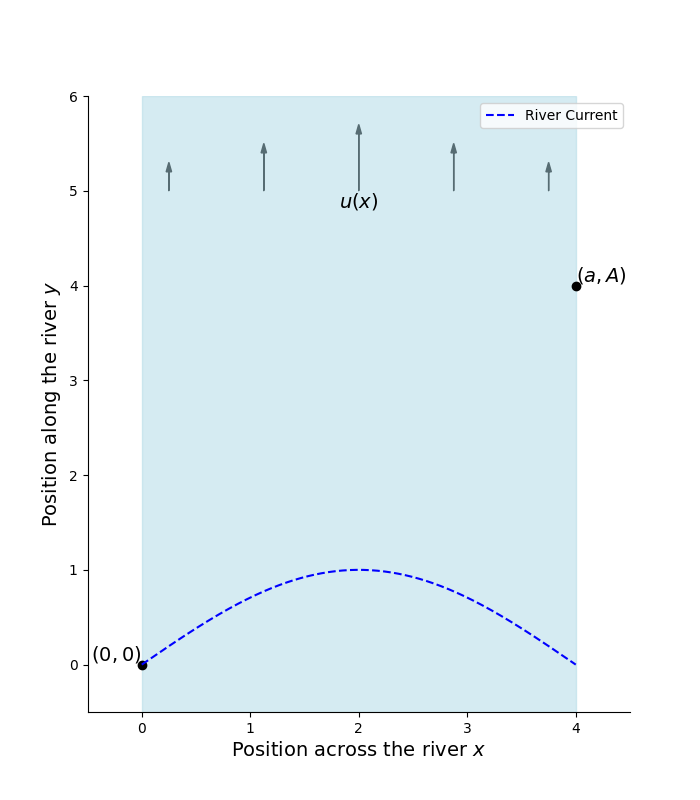
\includegraphics[width=\textwidth]{papers/schwimmen/Grafiken/Figure_2.png}	
        \caption{Flussströmung}
        \label{fig:no_velocity}
    \end{subfigure}
    \hfill  
    \begin{subfigure}{0.48\textwidth}
        \centering
        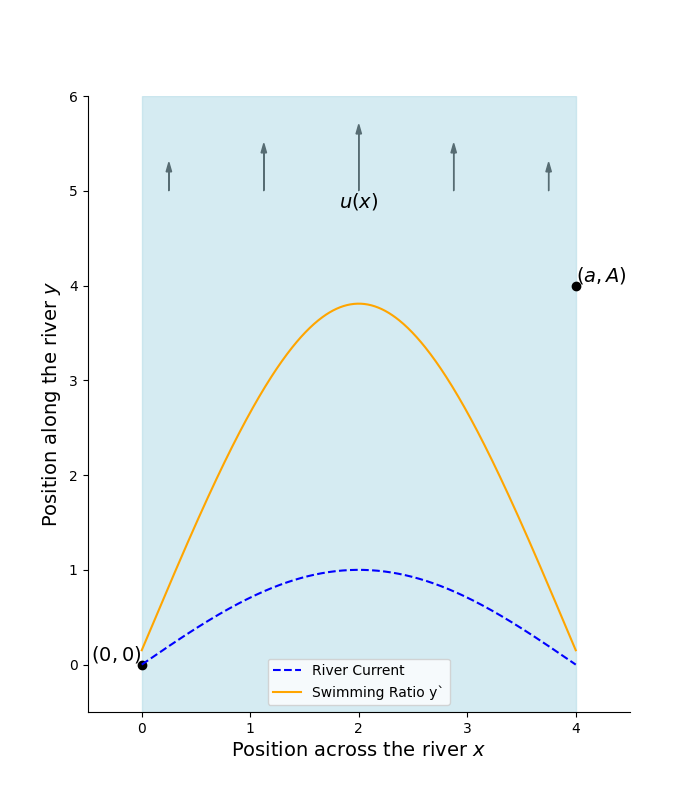
\includegraphics[width=\textwidth]{papers/schwimmen/Grafiken/Figure_3.png}	
        \caption{\(y' = \frac{dy}{dx}\)}
        \label{fig:diagonal_velocity}
    \end{subfigure}
    \par\bigskip
    \begin{subfigure}{0.48\textwidth}
        \centering
        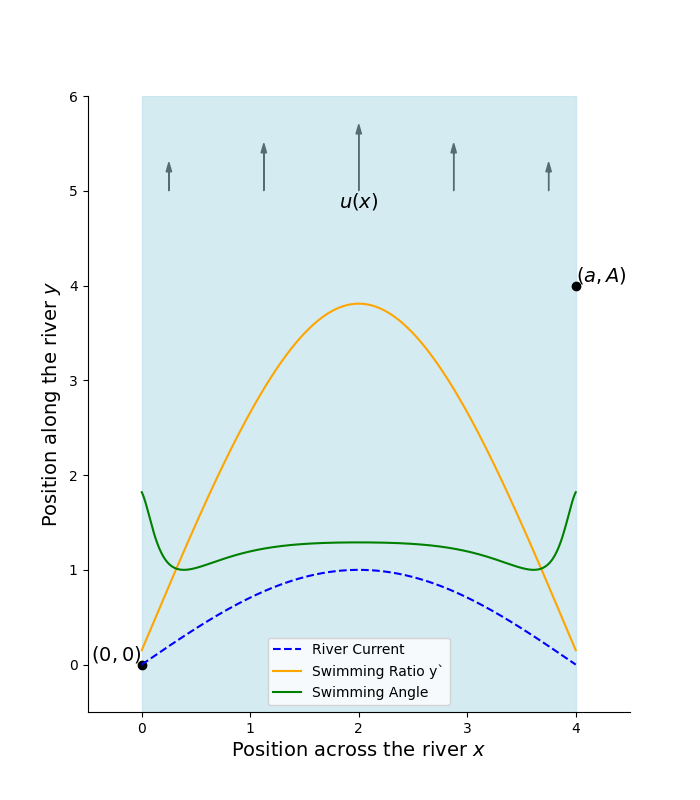
\includegraphics[width=\textwidth]{papers/schwimmen/Grafiken/Figure_4.png}	
        \caption{Winkel der Schwimmenden Person}
        \label{fig:squerd_velocity}
    \end{subfigure}
    \hfill  
    \begin{subfigure}{0.48\textwidth}
        \centering
        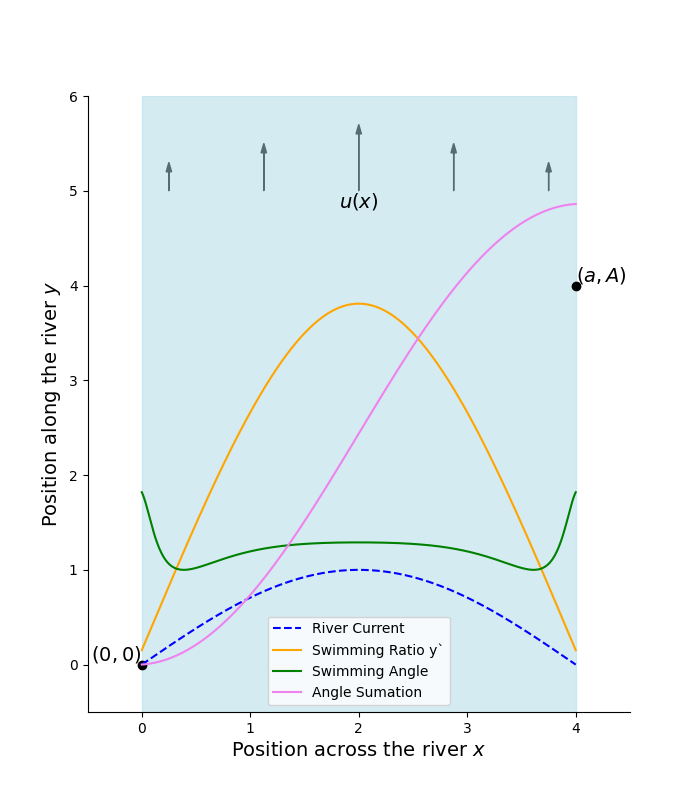
\includegraphics[width=\textwidth]{papers/schwimmen/Grafiken/Figure_5.png}	
        \caption{Aufsumierte Steigung}
        \label{fig:sin_velocity}
    \end{subfigure}
    \par\bigskip
    \caption{Die vier Grafiken stellen verschiedene Graphen dar die für die Flussüerquerung zentrall sind, \(a\) stellt die Flussströmung dar, \(b\) das Verhältis zwischen was in \(x\)- und \(y\)-Richtung geschwommen wird, \(c\) den Winkel der aus dem Verhältnis folgt und \(d\) das aufsumierte Verhältnis}
    \label{fig:river_pfrofiles}
\end{figure}




% Die Gleichung \ref{eq:angle} das Verhältnis \(\frac{dy}{dx}\) für die Richtung der schwimmenden h den Winkel, den man schwimmen sollte, um die optimale Flussüberquerung zu erreichen. Die beiden Schwimmgeschwindigkeiten \(c_y\) und \(c_x\) sind durch den Satz des Pythagoras miteinander verknüpft. Es ist definiert, dass die schwimmende Person durch ihre Schwimmleistung bzw. Schwimmkraft limitiert ist. Um diese Limitation zu berücksichtigen, wird festgelegt, dass die schwimmende Person nicht mehr Kraft hat, als sich mit der Geschwindigkeit \(v\) in ruhigem Wasser fortzubewegen. Durch diese Definition folgt, dass
% \begin{equation}
%     v^2 = c_y^2 + c_x^2
% \end{equation}
% gilt. Die Geschwindigkeit \(c_y\), die der Geschwindigkeit in Flussrichtung entspricht, ist äquivalent zur Strömungsgeschwindigkeit \(u\), da die Person auf der anderen Uferseite auf gleicher Höhe ankommen muss. Daraus ergibt sich
% \begin{equation}
%     c_x = \sqrt{v^2 - u^2}
% \end{equation}
% wobei, \(v\) eine Konstante ist die man frei wählen kann, ein Richtwert könnte \(1\,\mathrm{m/s}\) sein.
% In Abbildung \ref{fig:river_pfrofiles} sind die besten Schwimmmöglichkeiten dargestellt, um das andere Ufer zu erreichen. Das in Abbildung \ref{fig:sin_velocity} dargestellte Profil ist das realistischste und entspricht am ehesten den Gegebenheiten eines Flusses. Die anderen Flussprofile dienen der Veranschaulichung von Gedankenexperimenten.

% %papers/schwimmen/
% \begin{figure}
%     \centering
%     \begin{subfigure}{0.48\textwidth}
%         \centering
%         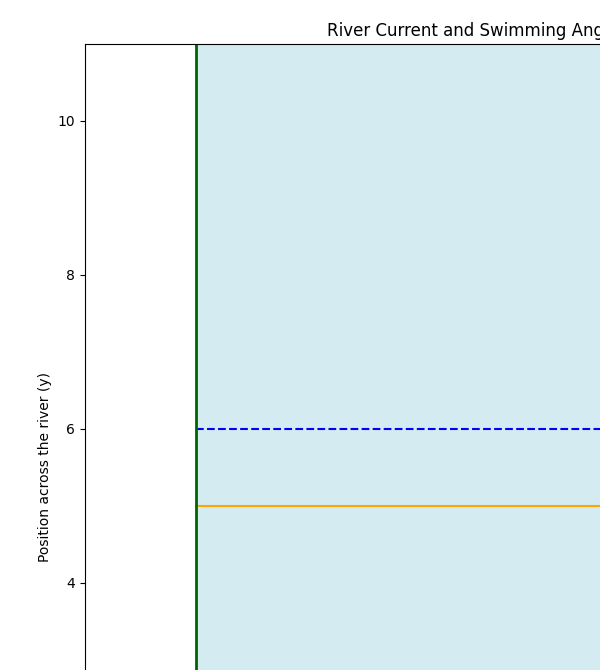
\includegraphics[width=\textwidth]{Grafiken/strait-crop.png}	
%         \caption{Stillstehender Fluss \newline}
%         \label{fig:no_velocity}
%     \end{subfigure}
%     \hfill  
%     \begin{subfigure}{0.48\textwidth}
%         \centering
%         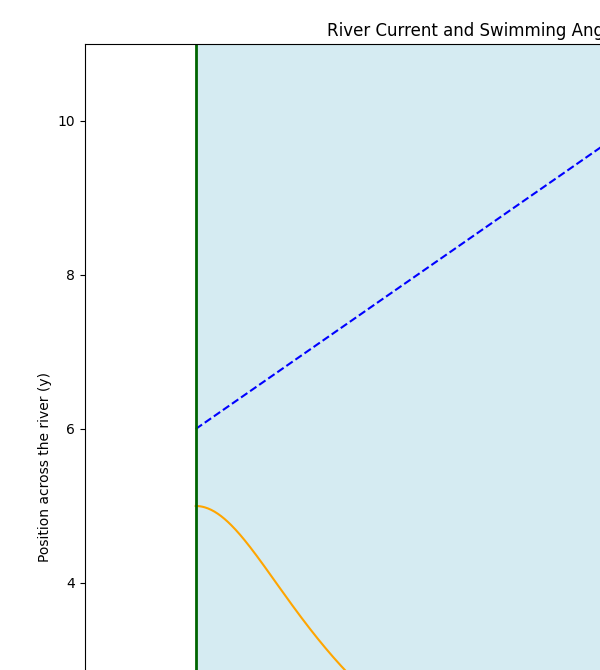
\includegraphics[width=\textwidth]{Grafiken/diagoal-crop.png}	
%         \caption{Lineares Flussgeschwindigkeitsprofil}
%         \label{fig:diagonal_velocity}
%     \end{subfigure}
%     \par\bigskip
%     \begin{subfigure}{0.48\textwidth}
%         \centering
%         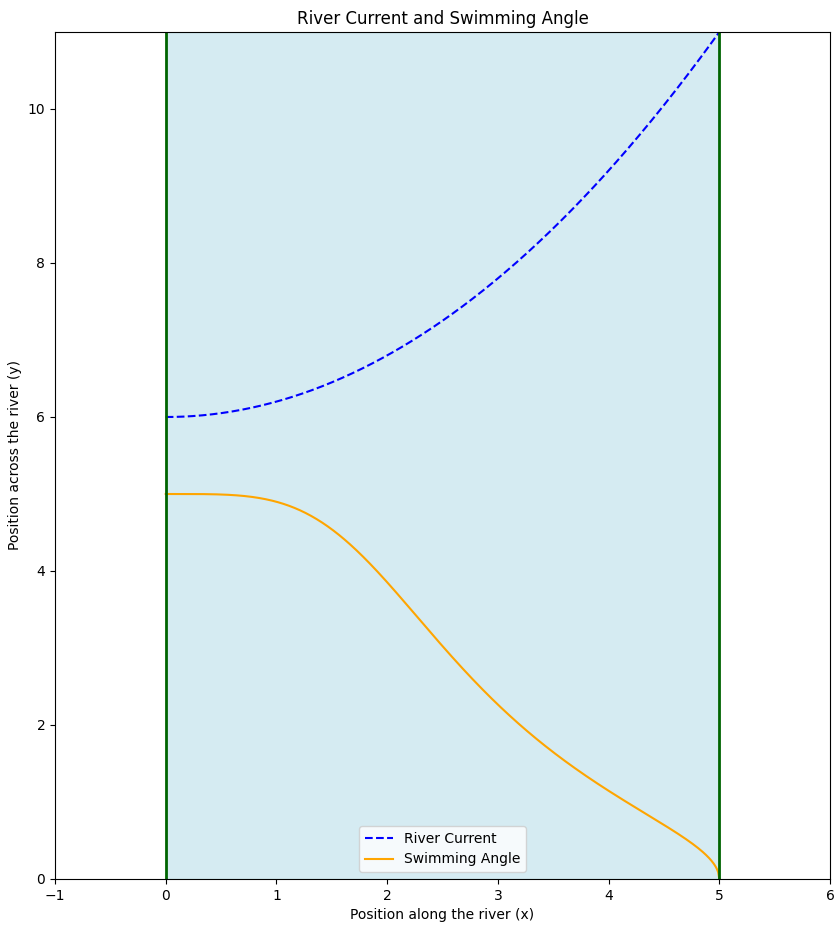
\includegraphics[width=\textwidth]{Grafiken/squard-crop.png}	
%         \caption{Quadratisches Flussgeschwindigkeitsprofil}
%         \label{fig:squerd_velocity}
%     \end{subfigure}
%     \hfill  
%     \begin{subfigure}{0.48\textwidth}
%         \centering
%         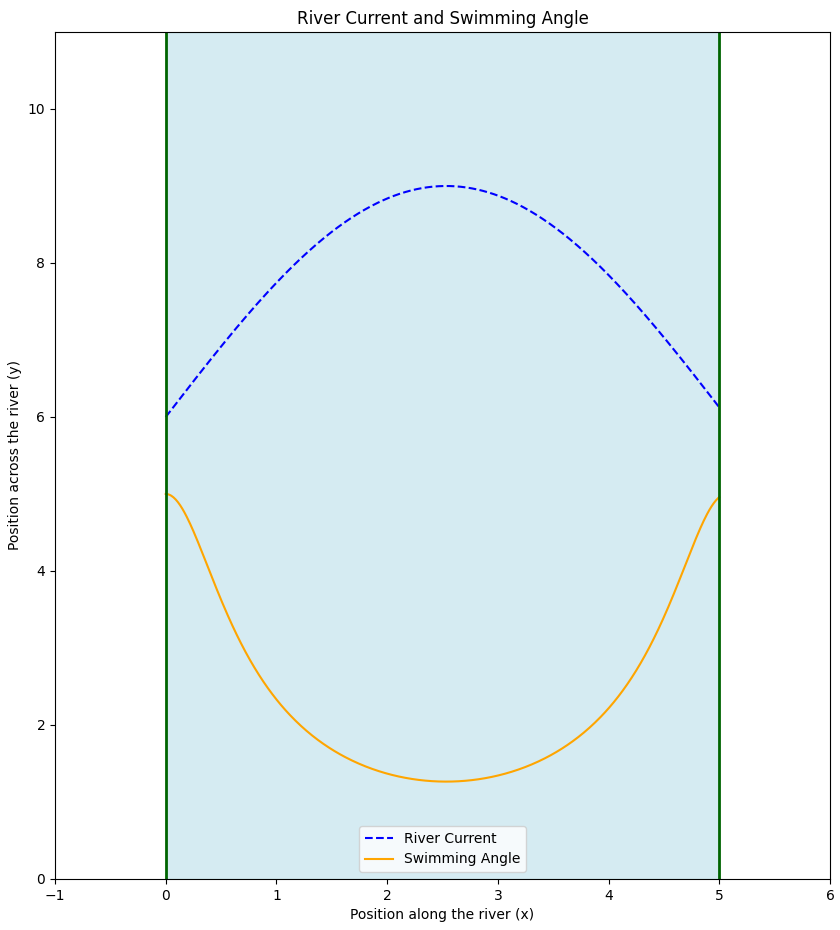
\includegraphics[width=\textwidth]{Grafiken/sin-crop.png}	
%         \caption{Sinusförmiges Flussgeschwindigkeitsprofil}
%         \label{fig:sin_velocity}
%     \end{subfigure}
%     \par\bigskip
%     \caption{Die vier Grafiken stellen jeweils einen Fluss mit dem entsprechenden Flussgeschwindigkeitsprofil in Orange und dem Schwimmwinkel in Blau dar. Es ist zu beachten, dass die Flussströmung von unten nach oben verläuft. Der Winkel ist so zu interpretieren, dass je flacher er verläuft (in \(x\)-Richtung), desto geradliniger bewegt man sich auf die andere Uferseite zu.}
%     \label{fig:river_pfrofiles}
% \end{figure}




















% Die Gleichung \ref{eq:angle} beschreibt den Winkel den man schwimmen sollte für die optimale Flussüberquerung. Die beiden Schwimmgeschwindigkeiten \(c_y\) und \(c_x\) sind von einander über den Satz des Pythagorases abhängig. Es ist definiert das der Mensch durch seine schwimmleistung bzw. schwimmkaraft limitiert ist. Um diese Limitation beizubehalten definiert man das der Mensch nicht mehr Kraft hat als sich mit der Geschwindigkeit \(v\) fortzubewegen (schwimmen). Durch diese Definition folgt das 
% \begin{equation}
%     v^2=c_y^2+c_x^2
% \end{equation}
% ist. Die \(c_y\) Geschwindigkeit die der Geschwindigkeit in Flussrichtung entspricht ist equivalent zur Strömungsgeschwindigkeit \(u\) da man auf der anderen Uferseite auf gleicher Höhe sein muss. In Abbildung \ref{fig:river_pfrofiles} siht man die besten schwimmmöglichkeiten um das andere Ufer zu erreichen. Das in \ref{fig:sin_velocity} dargestelle Profiel ist das realistischte übereinstimmende Profiel mit einem Fluss. Die anderen Flussprofiele dienen meist der Gedankenstütze.



% \begin{figure}[h]
%     \centering
%     \begin{subfigure}{0.48\textwidth}
%         \centering
%         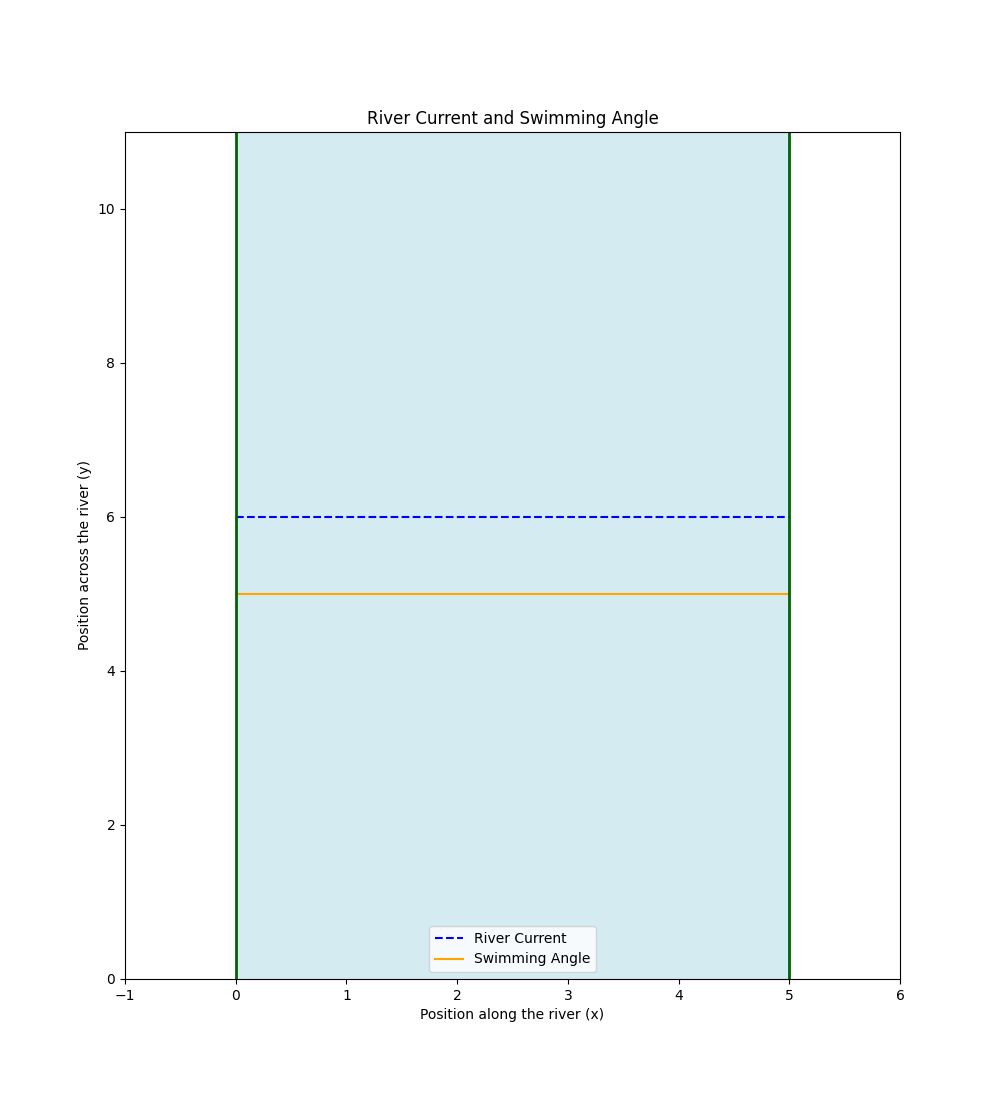
\includegraphics[width=1\textwidth]{Grafiken/strait.png}	
%         \caption{Stillstehender Fluss \newline}
%         \label{fig:no_velocity}
%     \end{subfigure}
%     \hfill  
%     \begin{subfigure}{0.48\textwidth}
%         \centering
%         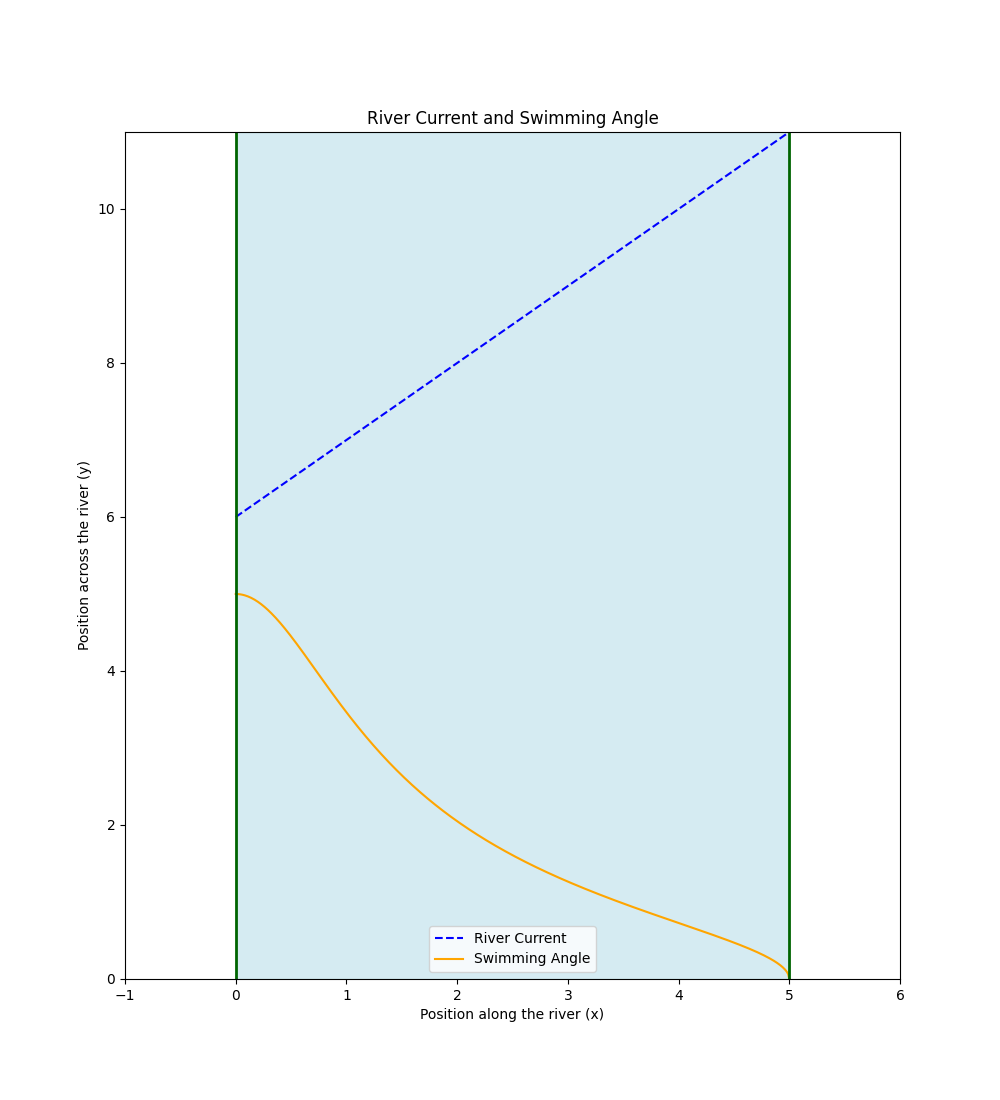
\includegraphics[width=1\textwidth]{Grafiken/diagoal.png}	
%         \caption{Diagonales Flussgeschwindigkeitsprofil}
%         \label{fig:diagonal_velocity}
%     \end{subfigure}
%     \par\bigskip
%     \begin{subfigure}{0.48\textwidth}
%         \centering
%         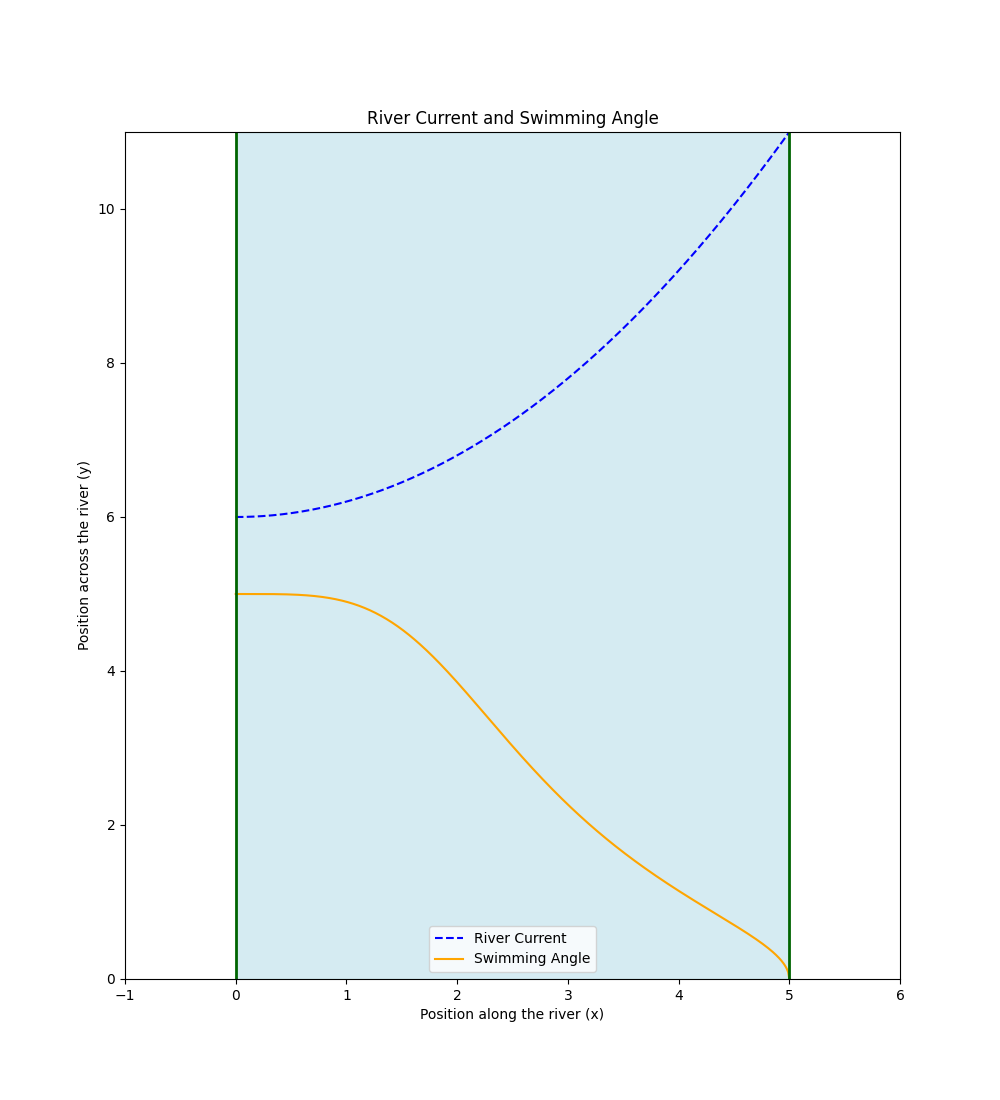
\includegraphics[width=1\textwidth]{Grafiken/squard.png}	
%         \caption{Quadratisches Flussgeschwindigkeitsprofil}
%         \label{fig:squerd_velocity}
%     \end{subfigure}
%     \hfill  
%     \begin{subfigure}{0.48\textwidth}
%         \centering
%         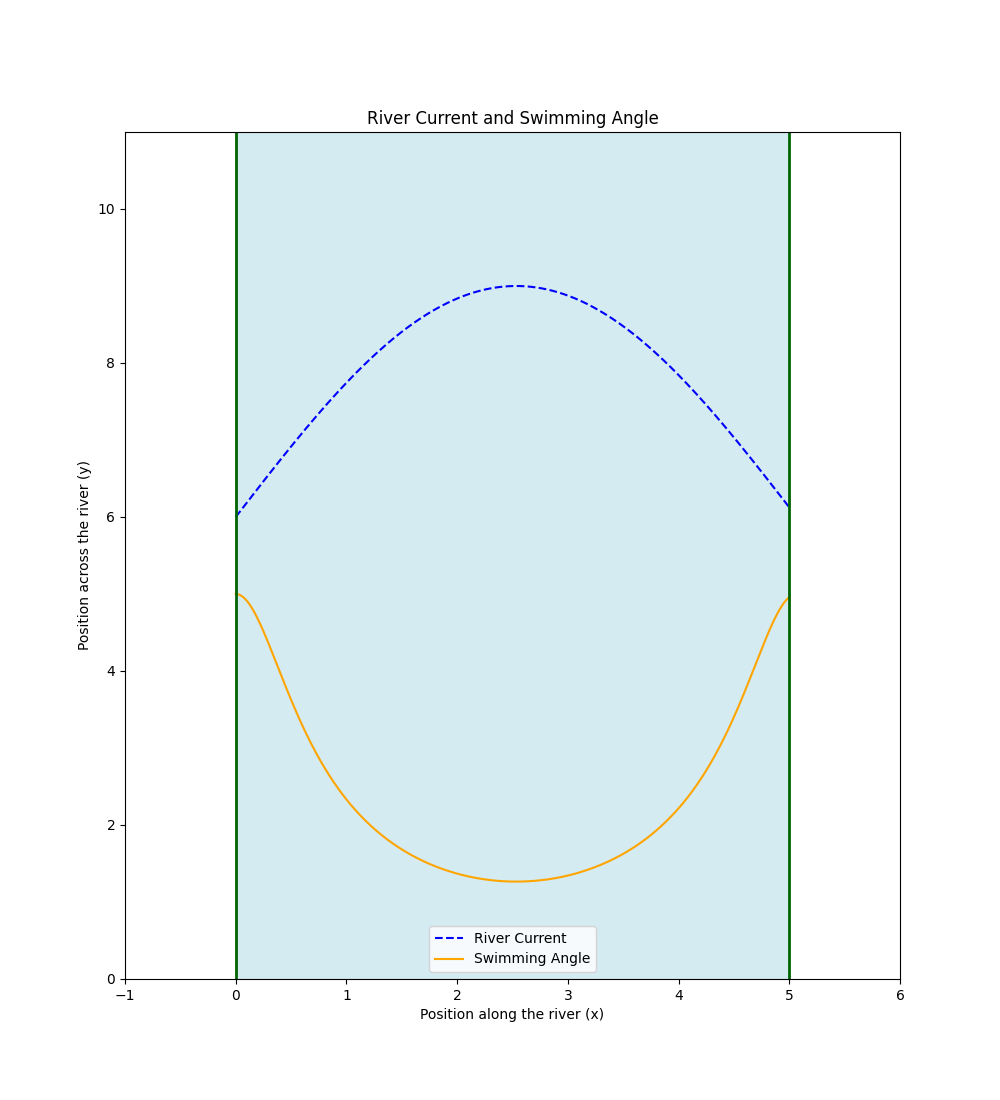
\includegraphics[width=1\textwidth]{Grafiken/sin.png}	
%         \caption{Sinusförmiges Flussgeschwindigkeitsprofil}
%         \label{fig:sin_velocity}
%     \end{subfigure}
%     \par\bigskip
%     \caption{Die vier Graphiken stellen immer einen Fluss dar mit dem jeweiligen Flussgeschwindigkeitsprofil in oragne und dem Schwimmwinkel in Blau. Es sei zu beachten das die Flussströmung von unten nach oben geht. Der Winkel ist so zu intepretieren das je Flächer (x Verhalten) er hat je gräder begiebt man sich auf die andere Uferseit}
%     \label{fig:river_pfrofiles}
% \end{figure}
